\documentclass{beamer}
\usepackage[utf8]{inputenc}
\usepackage[T1]{fontenc}
\usepackage[francais]{babel} 
\usepackage{lmodern}
\usepackage{hyperref}
\usepackage{pgfplots}
\usepackage{tikz}
\usepackage{algorithm2e}

\usetikzlibrary{trees,shapes.geometric,arrows,decorations.pathmorphing,backgrounds,fit,positioning,shapes.symbols,chains,patterns}
 \tikzset{
    %Define standard arrow tip
    >=stealth',
    %Define style for boxes
    punkt/.style={
           rectangle, dashed,
           rounded corners,
           draw=black, very thin,
           minimum height=2em,
           minimum width = 2cm,
           text centered},
    square/.style={
           rectangle,
           draw=black, thick,
           minimum height=.5cm,
           text centered},
    data/.style={
           rectangle,
           draw=black, thick,
           minimum height= 2cm,
           minimum width = 2cm,
           text centered},
    % Define arrow style
    pil/.style={
           ->,
           thick,
           shorten <=1pt,
           shorten >=1pt,},
    asym/.style={
           <->,
           thin,
           shorten <=1pt,
           shorten >=1pt,
           red!100},
    sym/.style={
           <->,
           thin,
           shorten <=1pt,
           shorten >=1pt,
           blue!100}
}


\usetikzlibrary{shapes.gates.logic.US,trees,positioning,arrows}
\tikzstyle{startstop} = [rectangle, rounded corners, minimum width=3cm, minimum height=1cm,text centered, draw=black, fill=red!30]
\tikzstyle{io} = [trapezium, trapezium left angle=70, trapezium right angle=110, minimum width=3cm, minimum height=1cm, text centered, draw=black, fill=blue!30]
\tikzstyle{process} = [rectangle, minimum width=3cm, minimum height=1cm, text centered, draw=black, fill=orange!30]
\tikzstyle{processH} = [rectangle, minimum width=1cm, minimum height=1cm, text centered, draw=black, fill=orange!30]
\tikzstyle{processS} = [rectangle, minimum width=1.3cm, minimum height=1.3cm, text centered, draw=black, fill=orange!30]
\tikzstyle{decision} = [diamond, minimum width=3cm, minimum height=1cm, text centered, draw=black, fill=green!30]
\tikzstyle{punkt} = [rectangle, dashed, rounded corners, draw=black, very thin,minimum height=2em,minimum width = 2cm, text centered]
\tikzstyle{arrow} = [thick,->,>=stealth]


\usepackage{eurosym}
\usepackage{rotating}
\usepackage{array}
\usepackage{multicol}
\usepackage{etex}
\usepackage{tikz-uml} 
\usepackage{amsmath}
\usepackage{amsfonts}

\usetheme{Antibes}
\usecolortheme{beaver}
\setbeamertemplate{sections/subsections in toc}[square]
\setbeamertemplate{blocks}[square]%

\setbeamercolor{footline}{fg=black}
\setbeamerfont{footline}{series=\bfseries}
\addtobeamertemplate{navigation symbols}{}{%
    \usebeamerfont{footline}%
    \usebeamercolor[fg]{footline}%
    \hspace{1em}%
    \insertframenumber/\inserttotalframenumber
}

\author{Claire Smets -- William Boisseleau -- Pascal Edouard -- \\Mathieu Latimier -- Julien Legras}
\title{Soutenance projet annuel\\ Audit des implantations SSL/TLS}
\titlegraphic{
\includegraphics[height=3em]{logo_univ.png}}
\institute{Master 2 Sécurité des Systèmes Informatiques}

\date{28/02/2014}

\setcounter{tocdepth}{1}
\begin{document}
{
\setbeamertemplate{headline}[default] 
\begin{frame}
  \titlepage
\end{frame}
}

%% 2 MIN -- PASCAL
\section*{Introduction}
\subsection{Sujet et problématique}
\frame{
\frametitle{Sujet et problématique I}

\begin{block}{Motivations}
	\begin{itemize}
		\item incertitudes cryptographiques liées aux récents scandales ;
		\item 2012 -- étude de l'Université du Michigan sur la sécurité d'internet : \textit{Mining your Ps and Qs: Widespread Weak Keys in Network Devices}
	\end{itemize}
\end{block}

\begin{center}
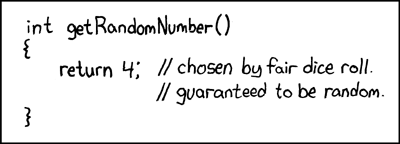
\includegraphics[height=7em]{images/random_number.png}
\end{center}
}

\frame{
\frametitle{Sujet et problématique II}
\begin{block}{Projet}
\begin{itemize}
\item mesure de l'évolution par rapport à cette étude;
\item identification des problèmes avérés;
\item audit de la principale bibliothèque : OpenSSL.
\end{itemize}
\end{block}

\begin{block}{Exigences du client}
\begin{itemize}
\item audit des certificats RSA;
\item quantité importante de données pour des résultats représentatifs (500 000 certificats).
\end{itemize}
\end{block}
}

\frame{
\frametitle{Sommaire}
\tableofcontents

}

%% PARTIE 1 - 16 MIN
\section{Audit des clefs RSA des certificats}

%% 4 MIN -- CLAIRE
\subsection{Récupération}
\subsubsection{Adresses}
\frame{
    \frametitle{Récupération des adresses}
{\footnotesize
\begin{center}
\begin{tikzpicture}[node distance=1.5cm]

\node[draw=none] (start) {};
\node[square, right=of start, fill=orange!30] (zmap) {ZMAP};
\node[square,right=of zmap] (applirc) {Appli RC};
\node[square,right=of applirc] (applif) {Appli F};
\node[draw=none] at (10,0) (end) {};

\draw (start) edge[->] node[midway,anchor=south] {port 443} (zmap);
\draw (zmap) edge[->] node[midway,anchor=south] (IP) {liste IP} (applirc);
\draw (applirc) edge[->] node[midway,anchor=south] {clefs} (applif);
\draw (applif) edge[->] node[midway,anchor=south] {facteurs} (end);
\draw (applif) edge[] node[midway,anchor=north] {communs} (end);

\begin{pgfonlayer}{background}
\node[punkt, fit=(start)(zmap)(IP)] {};
\end{pgfonlayer}

\end{tikzpicture}
\end{center}
}
    \begin{block}{ZMAP}
	\begin{itemize}
		\item open source dévoloppé en 2013 par l'équipe de l'Université du Michigan ;
		\item scanneur de ports : jusqu'à 1,4 millions de paquets SYN par seconde.\\
	\end{itemize}
	\end{block}
}

\subsubsection{Certificats}
\frame	{
    \frametitle{Récupération des certificats I}
    
    {\footnotesize
\begin{center}
\begin{tikzpicture}[node distance=1.5cm]

\node[draw=none] (start) {};
\node[square, right=of start] (zmap) {ZMAP};
\node[square,right=of zmap, fill=green!30] (applirc) {Appli RC};
\node[square,right=of applirc] (applif) {Appli F};
\node[draw=none] at (10,0) (end) {};

\draw (start) edge[->] node[midway,anchor=south] {port 443} (zmap);
\draw (zmap) edge[->] node[midway,anchor=south] (IP) {liste IP} (applirc);
\draw (applirc) edge[->] node[midway,anchor=south] (clefs) {clefs} (applif);
\draw (applif) edge[->] node[midway,anchor=south] {facteurs} (end);
\draw (applif) edge[] node[midway,anchor=north] {communs} (end);

\begin{pgfonlayer}{background}
\node[punkt, fit=(applirc)(clefs)(IP)] {};
\end{pgfonlayer}

\end{tikzpicture}
\end{center}
}
    
    
    %% Certificats + clefs
    \begin{block}{Récupération des certificats}
	\begin{itemize}
		\item commandes openssl pour établir la connexion SSL ;
		\item enregistrement de la session;
		\item extraction des certificats et des clefs RSA de la session SSL;
		\item élimination des doublons.
	\end{itemize}
	\end{block}
}



\frame{
    \frametitle{Gestion des doublons}
    
    {\footnotesize
\begin{center}
\begin{tikzpicture}[node distance=1.5cm]

\node[draw=none] (start) {};
\node[square, right=of start] (zmap) {ZMAP};
\node[square,right=of zmap, fill=green!30] (applirc) {Appli RC};
\node[square,right=of applirc] (applif) {Appli F};
\node[draw=none] at (10,0) (end) {};

\draw (start) edge[->] node[midway,anchor=south] {port 443} (zmap);
\draw (zmap) edge[->] node[midway,anchor=south] (IP) {liste IP} (applirc);
\draw (applirc) edge[->] node[midway,anchor=south] (clefs) {clefs} (applif);
\draw (applif) edge[->] node[midway,anchor=south] {facteurs} (end);
\draw (applif) edge[] node[midway,anchor=north] {communs} (end);

\begin{pgfonlayer}{background}
\node[punkt, fit=(applirc)(clefs)(IP)] {};
\end{pgfonlayer}

\end{tikzpicture}
\end{center}
}

	\begin{center}
\begin{tikzpicture}[level 1/.style={sibling distance=30mm},level 2/.style={sibling distance=10mm}]
\node {scan\_ssl}
    child {node {certs}
        child {node {ip.pem}}}
    child {node {certs\_links}
        child {node {hash}}}
    child {node {certs\_doublons}
        child {node {hash}}}
;
    
\end{tikzpicture}
\end{center}
}

\frame{
\frametitle{Certificats récupérés}

{\footnotesize
\begin{center}
\begin{tikzpicture}[node distance=1.5cm]

\node[draw=none] (start) {};
\node[square, right=of start] (zmap) {ZMAP};
\node[square,right=of zmap, fill=green!30] (applirc) {Appli RC};
\node[square,right=of applirc] (applif) {Appli F};
\node[draw=none] at (10,0) (end) {};

\draw (start) edge[->] node[midway,anchor=south] {port 443} (zmap);
\draw (zmap) edge[->] node[midway,anchor=south] (IP) {liste IP} (applirc);
\draw (applirc) edge[->] node[midway,anchor=south] (clefs) {clefs} (applif);
\draw (applif) edge[->] node[midway,anchor=south] {facteurs} (end);
\draw (applif) edge[] node[midway,anchor=north] {communs} (end);

\begin{pgfonlayer}{background}
\node[punkt, fit=(applirc)(clefs)(IP)] {};
\end{pgfonlayer}

\end{tikzpicture}
\end{center}
}

	\begin{block}{Certificats malformés}
		\begin{itemize}
			\item \textit{Common Name} vide : validation impossible au regard du nom de domaine ;
			\item \textit{Serial Number} seul : absence totale d'informations sur le certificat.\\
		\end{itemize}
	\end{block}
}


%% 5 MIN
% julien et william
\subsection{Factorisation}

\frame{
    \frametitle{Factorisation}
    \framesubtitle{Rappels sur la génération des clefs RSA}
    {\footnotesize
\begin{center}
\begin{tikzpicture}[node distance=1.5cm]

\node[draw=none] (start) {};
\node[square, right=of start] (zmap) {ZMAP};
\node[square,right=of zmap] (applirc) {Appli RC};
\node[square,right=of applirc, fill=green!30] (applif) {Appli F};
\node[draw=none] at (10,0) (end) {};

\draw (start) edge[->] node[midway,anchor=south] {port 443} (zmap);
\draw (zmap) edge[->] node[midway,anchor=south] (IP) {liste IP} (applirc);
\draw (applirc) edge[->] node[midway,anchor=south] (clefs) {clefs} (applif);
\draw (applif) edge[->] node[midway,anchor=south] (facteurs) {facteurs} (end);
\draw (applif) edge[] node[midway,anchor=north] {communs} (end);

\begin{pgfonlayer}{background}
\node[punkt, fit=(applif)(clefs)(facteurs)] {};
\end{pgfonlayer}

\end{tikzpicture}
\end{center}
}

\begin{block}{Algorithme de génération de clefs RSA}
\begin{enumerate}
\item générer $p$ et $q$ premiers et différents;
\item calculer $N = p \times q$ et $\phi(N)= (p-1)\times(q-1)$ (indicatrice d'Euler);
\item tirer aléatoirement $e \in \mathbb{Z}/\phi(N)\mathbb{Z}$;
\item calculer $d$ tel que $d \times e \equiv 1 \mod{\phi(N)}$;
\item $clef\, publique = N, e$ ; \textit{clef privée} $= p, q, d$
\end{enumerate}
\end{block}
}

\frame{
    \frametitle{Factorisation}
    \framesubtitle{Factorisation des clefs RSA}
    {\footnotesize
\begin{center}
\begin{tikzpicture}[node distance=1.5cm]

\node[draw=none] (start) {};
\node[square, right=of start] (zmap) {ZMAP};
\node[square,right=of zmap] (applirc) {Appli RC};
\node[square,right=of applirc, fill=green!30] (applif) {Appli F};
\node[draw=none] at (10,0) (end) {};

\draw (start) edge[->] node[midway,anchor=south] {port 443} (zmap);
\draw (zmap) edge[->] node[midway,anchor=south] (IP) {liste IP} (applirc);
\draw (applirc) edge[->] node[midway,anchor=south] (clefs) {clefs} (applif);
\draw (applif) edge[->] node[midway,anchor=south] (facteurs) {facteurs} (end);
\draw (applif) edge[] node[midway,anchor=north] {communs} (end);

\begin{pgfonlayer}{background}
\node[punkt, fit=(applif)(clefs)(facteurs)] {};
\end{pgfonlayer}

\end{tikzpicture}
\end{center}
}

\begin{block}{Factorisation de clefs RSA}
\begin{enumerate}
\item Algorithme naïf :
\begin{itemize}
\item calcul de PGCD deux à deux;
\item complexité : $O(n!)$.
\end{itemize}
\item Algorithme de Bernstein \textit{How to find smooth parts of integers?}
\begin{itemize}
\item structure arborescente;
\item complexité : $O(n\times lb(n))$.
\end{itemize}
\end{enumerate}
\end{block}
}


\frame{
    \frametitle{Factorisation}
    \framesubtitle{PGCD deux à deux}
\begin{center}
\begin{tikzpicture}
\begin{scope}[node distance=1cm,on grid,>=stealth',
		block/.style={rectangle,draw,fill=cyan!20},
		comp/.style={circle,draw,fill=orange!40},
		block2/.style={rectangle,draw,fill=orange!40}]	
		

	\node [block2] (N1)		[] {$N_1$};
	\node [block2] (N2)		[right=of N1,xshift=1.2cm] {$N_2$} ;
	\node [block2] (N3)		[right=of N2,xshift=1.2cm] {$N_3$} ;
	\node [block2] (N4)		[right=of N3,xshift=1.2cm] {$N_4$}  ;\pause	
	
	\node [block2] (N21) [below=of N1,xshift=+1.8cm] {$N_1N_2$} edge [<-] (N1) edge [<-] (N2) ;	
	\node [block2] (N22) [right=of N21,xshift=2cm] {$N_3N_4$} edge [<-] (N3) edge [<-] (N4) ;	\pause

	\node [block2] (P) [below=of N21,xshift=1.4cm] {$N_1N_2N_3N_4$} edge [<-] (N21) edge [<-] (N22);\pause
	
	\node [block2] (mod1) [below=of P,xshift=-1.4cm] {$\mod (N_1N_2)^2$}  edge [<-] (P); 
	\node [block2] (mod2) [right=of mod1,xshift=2cm] {$\mod (N_3N_4)^2$}  edge [<-] (P);\pause
	
	\node [block2] (mod21)		[below=of mod1,xshift=-1.8cm] {$\mod N_1^2$} edge [<-] (mod1);
	\node [block2] (mod22)		[right=of mod21,xshift=1.2cm] {$\mod N_2^2$} edge [<-] (mod1);
	\node [block2] (mod23)		[right=of mod22,xshift=1.2cm] {$\mod N_3^2$}  edge [<-] (mod2);
	\node [block2] (mod24)		[right=of mod23,xshift=1.2cm] {$\mod N_4^2$}  edge [<-] (mod2);\pause

	
	\node [block2] (div1)		[below=of mod21] {$/N_1$} edge [<-] (mod21);
	\node [block2] (div2)		[below=of mod22] {$/N_2$} edge [<-] (mod22);
	\node [block2] (div3)		[below=of mod23] {$/N_3$}  edge [<-] (mod23);
	\node [block2] (div4)		[below=of mod24] {$/N_4$}  edge [<-] (mod24);\pause

	\node	[block2]	(gcd1)	[below=of div1]	{$pgcd(.,N_1)$} edge [<-] (div1);
	\node	[block2]	(gcd2) [below=of div2]		{$pgcd(.,N_2)$} edge [<-] (div2);
	\node	[block2]	(gcd3) [below=of div3]		{$pgcd(.,N_3)$} edge [<-] (div3);
	\node	[block2]	(gcd4) [below=of div4]	 	{$pgcd(.,N_4)$} edge [<-] (div4);
\end{scope}

\end{tikzpicture}

\end{center}
}


\frame{
    \frametitle{Factorisation}
    \framesubtitle{Exemple}

\begin{center}
\begin{tikzpicture}[scale=0.9, every node/.style={scale=0.9}]
\begin{scope}[node distance=1cm,on grid,>=stealth',
		node/.style={transform shape},
		block/.style={rectangle,draw,fill=cyan!20},
		comp/.style={circle,draw,fill=orange!40},
		block2/.style={rectangle,draw,fill=orange!40}]	
		

	\node [block2] (N1)		[] {$6$};
	\node [block2] (N2)		[right=of N1,xshift=1.2cm] {$15$} ;
	\node [block2] (N3)		[right=of N2,xshift=1.2cm] {$77$} ;
	\node [block2] (N4)		[right=of N3,xshift=1.2cm] {$1$}  ;\pause	
	
	\node [block2] (N21) [below=of N1,xshift=+1.8cm] {$90$} edge [<-] (N1) edge [<-] (N2) ;	
	\node [block2] (N22) [right=of N21,xshift=2cm] {$77$} edge [<-] (N3) edge [<-] (N4) ;	\pause

	\node [block2] (P) [below=of N21,xshift=1.4cm] {$6930$} edge [<-] (N21) edge [<-] (N22);\pause
	
	\node [block2] (mod1) [below=of P,xshift=-3.2cm] {$\mod (90)^2 = 6930$}  edge [<-] (P); 
	\node [block2] (mod2) [below=of P,xshift=3.2cm] {$\mod (77)^2 = 1001$}  edge [<-] (P);\pause
	
	\node [block2] (mod21)		[below=of mod1,xshift=-1.5cm] {$\mod 6^2 = 18$} edge [<-] (mod1);
	\node [block2] (mod22)		[below=of mod1,xshift=1.5cm] {$\mod 15^2 = 180$} edge [<-] (mod1);
	\node [block2] (mod23)		[below=of mod2,xshift=-1.5cm] {$\mod 77^2 = 1001$}  edge [<-] (mod2);
	\node [block2] (mod24)		[below=of mod2,xshift=1.5cm] {$\mod 1^2 = -$}  edge [<-] (mod2);\pause

	
	\node [block2] (div1)		[below=of mod21] {$/6=3$} edge [<-] (mod21);
	\node [block2] (div2)		[below=of mod22] {$/15=12$} edge [<-] (mod22);
	\node [block2] (div3)		[below=of mod23] {$/77=13$}  edge [<-] (mod23);
	\node [block2] (div4)		[below=of mod24] {$-$}  edge [<-] (mod24);\pause
	
	\node	[block2]	(gcd1) [below=of div1]	{$pgcd(3,6)=3$} edge [<-] (div1);
	\node	[block2]	(gcd2) [below=of div2]		{$pgcd(12,15)=3$} edge [<-] (div2);
	\node	[block2]	(gcd3) [below=of div3]		{$pgcd(13,77)=1$} edge [<-] (div3);
	\node	[block2]	(gcd4) [below=of div4]	 	{$-$} edge [<-] (div4);
\end{scope}

\end{tikzpicture}

\end{center}
}


\frame[allowframebreaks=1]{
    \frametitle{Optimisations}
\begin{block}{Parallélisation}
En largeur avec 100 threads


    \begin{center}
\begin{tikzpicture}[level 1/.style={sibling distance=30mm},level 2/.style={sibling distance=10mm},scale=0.7,every node/.style={transform shape}]
\node (root) {$P$}  [grow=up]
  child {node {315}
  	child  {node [circle,draw] {21}}
  	child  {node [circle,draw] {15}}
  }
  child {node {?}
  	child {node [circle,draw] {63}}
  	child  {node [circle,draw] {22}}
  }
  child {node {?}
  	child {node [circle,draw] {35}}
  	child  {node [circle,draw] {91}}
  }
  child {node {2535}
  	child {node [circle,draw] {39}}
  	child  {node [circle,draw]{65}}
  } 
;
\end{tikzpicture}
\end{center}
\end{block}

\begin{alertblock}{Parallélisation}
  En hauteur : ralentissement du traitement à cause de la dépendances entre les niveaux
 \end{alertblock}

\framebreak
\begin{block}{Langage et bibliothèque}
C \& \textit{libGMP}
\end{block}

\begin{block}{Stockage}
\begin{itemize}
\item programme initial : utilisation de fichiers pour stocker chaque niveau;
\item programme amélioré : stockage de l'arbre des produits en RAM (4-5 Go pour 500 000 clefs).
\item[] $\Rightarrow$ jusqu'à 10 fois plus rapide même avec un SSD
\end{itemize}
\end{block}

\begin{block}{Calcul des carrés}
Préférer la fonction d'exponentiation de GMP plutôt que la multiplication
$\Rightarrow$ jusqu'à 5 fois plus rapide
\end{block}
}

\frame[containsverbatim]{
    \frametitle{Factorisation}
    \begin{center}
    \Huge Démonstration
    \newline
    \normalsize
    
    Jeu de données : \verb+15, 22, 437, 1189, 527, 21, 3233, 3827+
    \end{center}
}

%% 5 MIN -- PASCAL
\subsection{Bilan}
\frame{
    \frametitle{Bilan}
    
\begin{block}{Deux jeux de données}
\begin{enumerate}
\item clefs récupérées par notre script : 85 000;
\item clefs du projet Sonar  : 527 000 fin janvier \url{https://scans.io/stduy/sonar.rdns/}.
\end{enumerate}

\end{block}


\begin{block}{Traitement}
   	\begin{itemize}
   	    \item factorisation ;
   	    \item insertion dans une base de données;
		\item développement d'une interface web avec graphiques :
		\begin{enumerate}
		    \item 125 vulnérables (0,12\%);
		    \item 2 382 vulnérables (0,46\%) -- 40 de Cisco.
		\end{enumerate}
	\end{itemize}
\end{block}

}

\subsection{Démonstration}
\frame{
    \frametitle{Analyse d'un certificat vulnérable}
    \centering
    \includegraphics[width=9cm]{qualis_notation.jpg}
}

%% PARTIE 2 - 16 MIN
\section{Audit d'OpenSSL}
\frame{
%% 1 MIN -- CLAIRE
\frametitle{Introduction I}
\begin{block}{OpenSSL}
API libre implémentant des primitives cryptographiques et le protocole SSL/TLS.
\newline
\textbf{450 000 lignes de code}.
\end{block}

\begin{block}{Historique d'OpenSSL}
\begin{itemize}
\item SSLeay développé par Eric Young \& Tim Hudson chez Cryptosoft;
\item 1998 -- passation du projet à la communauté : OpenSSL;
\item 6 janvier 2014 -- version 1.0.1f.
\end{itemize}
\end{block}
}

\frame{
    \frametitle{Introduction II}
	\begin{block}{Contexte}
	\begin{itemize}
		\item origine de vulnérabilité des certificats ;
		\item contexte actuel : sentiment d'incertitude ;
		\item beaucoup d'outils utilisés. \\
	\end{itemize}
	\end{block}
	\begin{block}{Audit d'OpenSSL}
		Trois grands axes : 
		\begin{itemize}
			\item la génération de l'aléatoire ;
			\item la génération des clefs ;
			\item le protocole SSL/TLS.\\
		\end{itemize}
	\end{block}
}

\frame{
\frametitle{Méthodologie de recherche de failles}
	\begin{block}{Où ?}
		\begin{itemize}
			\item site des CVE mitre;
			\item site de Vigil@nce ;
			\item RFC et standards.\\
		\end{itemize}
	\end{block}
	
	\begin{block}{Corrections ?}
		Présence de corrections? Si oui, lesquelles et par qui?
	\end{block}
}


%% 4 MIN -- WILLIAM (3 MIN)
\subsection{Générateur aléatoire}
%% 2 MIN -- MATHIEU

\frame{
\frametitle{Génération des clefs}
\begin{block}{Principes de Kerckhoffs}
	\begin{itemize}
	\item le \textit{secret} réside dans la clef ;
	\item les algorithmes de génération de clefs ne doivent donner aucune information sur la clef.
	\end{itemize}
\end{block}

\begin{center}
\begin{tikzpicture}[node distance=.1cm]
\node[draw, text width=2cm] (genalea1) {Générateur aléatoire};
\node[below=of genalea1, yshift=-1cm] (clefsym) {Clef symétrique};
\draw (genalea1) edge[->] (clefsym) ;

\node[draw, text width=2cm, right=of genalea1, xshift=1cm] (genalea2) {Générateur aléatoire};
\node[right=of genalea2] (plus) {+};
\node[draw, text width=3cm,right=of plus] {Structure mathématique};
\node[below=of plus, yshift=-1.2cm] (clefasym) {Clef asymétrique};
\draw (plus) edge[->] (clefasym);

\end{tikzpicture}
\end{center}

}

\frame{
\frametitle{Générateur aléatoire}
\framesubtitle{Définitions}


\begin{block}{Générateur}
\begin{itemize}

\item problème aléatoire ;
\item mesure de l'entropie : $H(X) = - \sum_x P(X=x)\times\log_2(P(X=x))$ (exprimée en Shannon) :
\begin{itemize}
\item si la VA est équirépartie alors l'entropie est maximale;
\item sinon inférieure à 50\%.
\end{itemize}
\item entropie et moduli.

\end{itemize}
\end{block}
	
}


\frame{
\frametitle{Entropie}
\vspace*{-1cm}
\begin{center}
\begin{tikzpicture}[scale=0.75, every node/.style={scale=0.75},node distance=1.5cm]
\node (donnees) [io,pattern=dots,pattern color=orange] {Données};
\node (bruit) [below=of donnees, yshift=1.9cm] {BRUIT};
\node (digit) [process, right of=donnees, xshift=4cm] {Numérisation};
\node (cond) [process, below of=digit,text width=3cm,yshift=-1.5cm] {Traitement (optionnel)};
\node (bat) [process, right of=cond, xshift=4cm] {Batterie de tests}; 
\node (dec) [decision, below of=cond,yshift=-1.2cm] {Sortie}; 
\node (appli) [process, below of=dec, yshift=-1cm] {Application};

\begin{pgfonlayer}{background}
\node[punkt, fit=(donnees)(digit)(cond)(bat)(dec), fill=yellow!5] (groupclient) {};
\end{pgfonlayer}

\begin{pgfonlayer}{background}
\node[punkt, fit=(donnees)(digit)(bruit), fill=yellow!20] (groupclient) {};
\end{pgfonlayer}

\draw [arrow] (donnees) -- (digit);
\draw [arrow] (digit) -- node[anchor=east] {out1}(cond);
\draw [arrow] (cond) -- node[anchor=east] {out2} (dec);
\draw [arrow] (digit) -| node[anchor=south] {out1} (bat);
\draw [arrow] (cond) -- node[anchor=south] {out2} (bat);
\draw [arrow] (bat) |- node[anchor=north] {true/false} (dec);
\draw [arrow] (dec) -- node[anchor=east] {output/error} (appli);
\end{tikzpicture}
\end{center}
}


\frame{
\frametitle{Entropie}

\begin{block}{Tests}
\begin{itemize}
\item tests trop anciens, \texttt{FIPS 140-1} (1994), non mis à jour :
 	\begin{itemize}
 	\item test monobit;
	\item test poker;
	\item test runs;
	\item test long runs.
	\end{itemize}
\item[$\hookrightarrow$] adaptation des tests obsolètes (20 000 à 8 000 000 bits) développés par l'équipe d'OpenSSL;
\item autres tests proposés dans le rapport (NIST).  

\end{itemize}
\end{block}
		
	
}


%% MATHIEU (1 MIN)
\frame[containsverbatim]{
\frametitle{Entropie -- Démonstration}
\begin{block}{Faille générateur d'aléatoire sur clefs RSA}
\begin{itemize}
\item version : OpenSSL 0.9.8 (2008) sous Debian 4.0;
\item but : retrouver la clef privée d'un certificat;
\item moyens : bibliothèque OpenSSL, \verb+openssl-vulnkey+, liste des 250 000 facteurs premiers possibles;
\item cause : suppression d'une grande source d'entropie dans \verb+crypto/rand/md_rand.c+;
\item impactés : IBM \& CISCO (sur le premier scan).
\end{itemize}
\end{block}

\begin{block}{Failles similaires -- 2013}
\begin{itemize}
\item Android / Linux Mint Debian Edition
\item NetBSD 6.0 et OpenSSH
\end{itemize}
\end{block}
}

\subsection{Génération des clefs I}

\frame[containsverbatim]{
\frametitle{Génération des clefs II}
\begin{block}{Attaque Man in the middle sur Diffie-Hellman}
\begin{itemize}
\item but : déchiffrer les messages entre un client et un serveur en forçant la génération d'un secret DH;
\item moyens : 
\begin{itemize}
\item mode FIPS activé sous OpenSSL;
\item écoute active sur le réseau.
\end{itemize}
\item cause : génération d'un faux positif lors d'un test dans \verb+crypto/dh/dh_key.c+
\end{itemize}
\end{block}
}

%% 3 MIN -- JULIEN
\subsection{Chiffrement et protocole SSL/TLS}
\frame[containsverbatim]{
\frametitle{Chiffrement}
\begin{block}{Timing attack sur RSA-OAEP}
\begin{itemize}
\item version : OpenSSL 1.0.0 (2010);
\item but : retrouver la clef privée d'un certificat en contrôlant la taille des paramètres à hacher;
\item moyens : RSA-OAEP, variations de délais;
\item impact :
\begin{itemize}
\item théorique sur les serveurs;
\item pratique sur les systèmes embarqués.
\end{itemize} 
\end{itemize}
\end{block}
}

\frame[allowframebreaks=1]{
\frametitle{Protocole SSL/TLS}

\begin{center}
\begin{tikzpicture}[remember picture,scale=0.6,every node/.style={transform shape}]
\begin{umlseqdiag} 
\umlobject[class=Client SSL/TLS] {C};
\umlobject[class=Serveur SSL/TLS,x=10] {S};

\begin{umlcall}[op={hello client},return={hello serveur},padding=2]{C}{S}\end{umlcall}

\begin{umlfragment}[type=alt, label=si certificat, inner xsep=10] 
\begin{umlcall}[dt=5,padding=2,op={certificat serveur},return={}]{S}{C}\end{umlcall}
\umlfpart[sinon]
\begin{umlcall}[op={clef publique serveur},return={},padding=2]{S}{C}\end{umlcall}
\end{umlfragment}

\begin{umlcall}[dt=4,padding=3,op={${\{master key\}}_{pk\,serveur}$},return={}]{C}{S}\end{umlcall}

\begin{umlcall}[dt=4,padding=3,op={${\{id\,connexion\}}_{masterkey'}$},return={${\{challenge\,hello\,client\}}_{masterkey''}$}]{C}{S}\end{umlcall}

\begin{umlcall}[dt=4,padding=3,op={${\{id\,session\}}_{masterkey'''}$},return={}]{S}{C}\end{umlcall}

\begin{umlcall}[dt=4,padding=3,op={Changement de l'algorithme de chiffrement du client},return={Changement de l'algorithme de chiffrement du serveur}]{C}{S}\end{umlcall}

\end{umlseqdiag} 
\end{tikzpicture}
\end{center}

\framebreak

\begin{block}{Historique}
\begin{itemize}
\item SSL 1.0 et 2.0 (1995) conçues par Netscape, 3.0 (1996) par l'IETF;
\item TLS 1.0 (1999) : légère amélioration de SSL 3, ajout d'extensions;
\item TLS 1.1 (2006) : protection contre les attaques contre CBC;
\item TLS 1.2 (2008) : remplacement MD5/SHA1 par SHA256, ajout des modes GCM et CCM.
\end{itemize}
\end{block}

}

\frame{
\frametitle{Failles notables d'OpenSSL}
SSL 3 et TLS 1.0:
\begin{itemize}
\item 2002 - attaque sur le padding du mode CBC par Serge Vaudenay (reprise par Lucky Thirteen): \textit{timing attack};
\end{itemize}
TLS 1.1 :
\begin{itemize}
\item \textbf{2011} (CVE-2011-4576) - récupération d'informations sur un échange précédent : mémoire non réinitialisée;
\item \textbf{2013} (CVE-2013-0169)- Lucky Thirteen : \textit{timing attack}, $2^{23}$ sessions TLS pour retrouver un bloc en clair;
\end{itemize}
TLS 1.2 :
\begin{itemize}
\item \textbf{2013} (CVE-2013-6449) - déni de service en envoyant une structure mal formée causant un \textit{crash} dans la fonction \texttt{ssl\_get\_algorithm2}
\end{itemize}
}

\frame[containsverbatim]{
\frametitle{Attaque à clair choisi en man in the middle}
\begin{block}{Attaque à clair choisi en man in the middle}
\begin{itemize}
\item versions : toutes;
\item but : déchiffrement du cookie de session;
\item moyens : \textit{cipersuite} en TLS 1.0 ou SSL 3.0 en mode de chiffrement CBC;
\item logiciel : BEAST.
\end{itemize}
\end{block}
}

%% 2 MIN -- JULIEN
\subsection{Ouverture}
\frame[containsverbatim]{
\frametitle{Remarques}

	    \begin{alertblock}{Points négatifs}
	        \begin{itemize}
	        \item documentation peu fournie;
	        \item développement en mode réactif;
	        \item illisibilité du code :
	        \begin{verbatim}
				n=((p[0]&0x7f)<<8)|p[1];				
			\end{verbatim}
	        \end{itemize}
	    \end{alertblock}
	\begin{exampleblock}{Points positifs}
		\begin{itemize}
			\item nom des fichiers standardisé : 
			\verb+s3_+ ;
			\item commentaires des commits.\\
		\end{itemize}
	\end{exampleblock}
}

\frame{
\frametitle{Ouverture}

\begin{block}{Alternatives}
\begin{itemize}
\item CyaSSL;
\item GnuTLS;
\item MatrixSSL;
\item Network Security Services	(Firefox);
\item PolarSSL (pas de support du DTLS);
\item Java Secure Socket Extension (pas de support du DTLS).
\end{itemize}
\end{block}

\begin{alertblock}{Attention -- 25 février 2014}
CVE-2014-1959 dans GnuTLS : validation de certificat (X509 version 1) intermédiaire comme un certificat d'AC par défaut.
\end{alertblock}

}


%% PARTIE 3  - 8 MIN
\section{Analyse dynamique du navigateur client}
%% 2 MIN 30 -- WILLIAM
\subsection{Faiblesses identifiées}
\frame[allowframebreaks=1]{
\frametitle{Faiblesses identifiées}
\begin{center}
\begin{tikzpicture}[node distance=0cm]
\node (Client) at (-5,0) {
\includegraphics[width=1.5cm]{computer}};
\node[below=of Client] (labC) {Client};
\node (Serveur) at (0,0) {
\includegraphics[width=1cm]{server}};
\node[below=of Serveur] (labS) {Serveur};

\draw (Client.north east) edge[->,bend left=20]  node[midway, anchor=south]{demande d'analyse} (Serveur.north west);

%\draw (Serveur.east) edge[->, loop right = 90] node[midway, anchor=west]{analyse} (Serveur.east);

\path (Serveur) edge[ out=30, in=-30
                , loop
                , distance=2cm, ->]
            node[anchor=west] {analyse} (Serveur);
            
\draw (Client.south east) edge[<-,bend right=20]  node[midway, anchor=north]{page de résultats} (Serveur.south west);

\end{tikzpicture}
\end{center}
\begin{block}{Critères}
\begin{itemize}
\item version du protocole;
\item \textit{ciphersuites} proposées par le client ;
\item courbes elliptiques supportées ;
\item algorithmes de signature ;
\item compression TLS;
\item activation ou non du ticket de session.
\end{itemize}
\end{block}

}




%% 2 MIN 30 --  JULIEN
\subsection{Implémentation}
\frame[allowframebreaks=1]{
\frametitle{Implémentation}

\begin{block}{Architectures possibles}
\begin{enumerate}
\item journalisation de la connexion HTTPS avec une sonde IDS puis récupération des informations avec un langage tel que PHP $\rightarrow$ couche réseau;
\item serveur HTTPS avec \textit{libssl} puis analyse de la structure de la session $\rightarrow$ couche applicative.
\end{enumerate}
\end{block}
\framebreak
\begin{center}
\begin{tikzpicture}[remember picture,scale=0.58,every node/.style={transform shape}]
\begin{umlseqdiag} 
\umlobject[class=Navigateur] {C};
\umlobject[class=Serveur HTTPS,x=7] {S};

\begin{umlcall}[dt=4,op={TCP connect},return={TCP accept},padding=4]{C}{S}\end{umlcall}

\begin{umlcall}[dt=4,op={SSL connect},return={SSL accept},padding=4]{C}{S}\end{umlcall}

\begin{umlcall}[dt=4,op={GET /site/analyze HTTP/1.0},return={code HTML}]{C}{S}

\begin{umlcallself}[op={Récupérer version du protocole}]{S}\end{umlcallself} 
\begin{umlcallself}[op={Récupérer support de la compression TLS}]{S}\end{umlcallself} 
\begin{umlcallself}[op={Récupérer ciphersuite cliente}]{S}\end{umlcallself} 
\begin{umlcallself}[op={Récupérer algorithmes de signature clients}]{S}\end{umlcallself} 
\begin{umlcallself}[op={Récupérer courbes elliptiques clientes}]{S}\end{umlcallself} 
\begin{umlcallself}[op={Récupérer support ticket TLS}]{S}\end{umlcallself} 

\end{umlcall}

\end{umlseqdiag} 
\end{tikzpicture}
\end{center}
}

%% 2 MIN -- MATHIEU
\subsection{Démonstration}
\frame{
\frametitle{Démonstration}
\begin{block}{Analyse de la sécurité des navigateurs clients}
\begin{itemize}
%% Chrome
\item Sous le navigateur graphique \texttt{Chrome} : le plus utilisé dans le monde.
%% Lynx  
\item Sous le navigateur console \texttt{lynx} : apprécié chez les développeurs.\newline
\end{itemize}
\end{block}

\begin{block}{Modification manuelle}
Nous pouvons modifier la \textit{ciphersuite} du client avec la commande \texttt{s\_client}.
\end{block}
}

%% 2 MIN -- PASCAL
\section{Conclusion}
\frame{
\frametitle{Conclusion}
\begin{block}{Bilan du projet -- \url{https://github.com/RandomGuys/}}
	\begin{itemize}
		\item Appli RC : récupération de certificats RSA;
		\item Appli F : factorisation de clefs RSA;
		\item site web :
		\begin{itemize}
		    \item statistiques;
		    \item analyse dynamique navigateur.
		\end{itemize}
		\item rapport d'audit.
	\end{itemize}
\end{block}

\begin{block}{Apports du projet}
	\begin{itemize}
		\item recherche approfondie de normes;
		\item riche en développement et en recherche.\\
	\end{itemize}
\end{block}
}

\frame{
\centering
\huge Questions ?
}
\end{document}
